\documentclass[11pt, a4paper]{article}

\usepackage[utf8]{inputenc}
\usepackage{graphicx}
\usepackage{amsmath}
\usepackage{amsfonts}
\usepackage{amssymb}
\usepackage{geometry}
\usepackage[
    backend=biber,
    style=ieee,
    citestyle=numeric-comp,
    sorting=none
]{biblatex}
\usepackage{hyperref}
\usepackage{caption}
\usepackage{subcaption}
\usepackage{booktabs}
\usepackage{float}
\usepackage{listings}
\usepackage{xcolor}
\usepackage{titlesec}
\usepackage{lmodern} % For better font rendering
\usepackage{fancyhdr}
\usepackage{titling}
\usepackage{enumitem} % For more control over lists

% Color scheme
\definecolor{primary}{RGB}{25,118,210}    % A nice blue
\definecolor{secondary}{RGB}{48,63,159}   % A darker indigo/blue
\definecolor{accent}{RGB}{216,27,96}      % A vibrant pink/magenta
\definecolor{lightgray}{RGB}{230,230,230} % Light gray for frames/backgrounds
\definecolor{darktext}{RGB}{50,50,50}     % Dark gray for body text

% Page geometry
\geometry{a4paper, margin=1in, headheight=15pt, footskip=30pt}

% Title formatting
\pretitle{\begin{center}\Huge\bfseries\color{secondary}} % Made title larger
\posttitle{\par\end{center}\vskip 1em} % Increased space after title
\preauthor{\begin{center}\Large\color{primary}} % Made author larger
\postauthor{\end{center}\vskip 0.5em}
\predate{\begin{center}\large\color{primary}}
\postdate{\end{center}}

% Section formatting
\titleformat{\section}
  {\normalfont\Large\bfseries\color{secondary}}
  {\thesection.}{0.5em}{} % Added a period after section number and reduced space slightly
\titleformat{\subsection}
  {\normalfont\large\bfseries\color{secondary}}
  {\thesubsection.}{0.5em}{} % Added a period
\titleformat{\subsubsection}
  {\normalfont\normalsize\bfseries\color{primary}}
  {\thesubsubsection.}{0.5em}{} % Added a period

% Header and footer
\pagestyle{fancy}
\fancyhf{} % Clear all header and footer fields
\fancyhead[L]{\small\color{primary}\leftmark}
\fancyhead[R]{\small\color{primary}Page \thepage}
\fancyfoot[C]{\small\color{gray}\textit{ResNet-32 on EuroSAT}} % Example footer
\renewcommand{\headrulewidth}{0.4pt}
\renewcommand{\footrulewidth}{0.4pt} % Added a footrule
\renewcommand{\headrule}{\hbox to\headwidth{\color{secondary}\leaders\hrule height \headrulewidth\hfill}}
\renewcommand{\footrule}{\hbox to\headwidth{\color{secondary}\leaders\hrule height \footrulewidth\hfill}}


% Abstract styling
\renewenvironment{abstract}
  {\begin{center}\large\bfseries\color{secondary}\abstractname\end{center}\vspace{0.5em} % Made abstract title larger
   \begin{quotation}\small\color{darktext}\noindent} % Ensured abstract text is dark
  {\end{quotation}}

% Code block styling (if you use it for code snippets)
\lstset{
    basicstyle=\ttfamily\footnotesize\color{darktext},
    breaklines=true,
    frame=tb, % Top and bottom frame lines
    rulecolor=\color{lightgray},
    backgroundcolor=\color{black!5}, % Very light gray background
    commentstyle=\color{green!60!black},
    keywordstyle=\color{blue!80!black}\bfseries,
    stringstyle=\color{red!80!black},
    numbers=left,
    numberstyle=\tiny\color{gray},
    stepnumber=1,
    numbersep=8pt,
    tabsize=2,
    showstringspaces=false
}

% Hyperref setup
\hypersetup{
    colorlinks=true,
    linkcolor=primary,
    filecolor=accent,
    urlcolor=secondary,
    pdftitle={Implementation and Evaluation of ResNet-32 for EuroSAT Image Classification},
    pdfpagemode=UseOutlines, % Shows bookmarks panel by default
    pdfauthor={Your Name Here},
}

\addbibresource{cite.bib} % Your .bib file name

\title{\textbf{Implementation and Evaluation of ResNet-32\\ for EuroSAT Image Classification}}
\author{ESUBALEW CHEKOL MULUYE \\ \textit{Deep Learning/GSR/6451/17}} % Replace with your details
\date{\today}

\begin{document}

% Title page
\begin{titlingpage}
    \maketitle
    \begin{abstract}
    Deep Convolutional Neural Networks (CNNs) have significantly advanced the field of image recognition. However, training exceptionally deep networks has historically been challenging due to issues like the degradation problem, where increased depth paradoxically leads to decreased performance. The ResNet (Residual Network) architecture, introduced by He et al. \cite{he2015deepresiduallearningimage}, effectively addressed this by employing a deep residual learning framework. This report details the implementation of a ResNet-32 model, a variant of this architecture, its training on the EuroSAT satellite imagery dataset, and an evaluation of its performance. We briefly cover the core principles of residual learning, the specifics of our ResNet-32 implementation, the data preparation pipeline for EuroSAT (a 10-class land use/land cover dataset), and the training strategies employed, including learning rate warmup and adaptive scheduling. The model's performance is analyzed through training/validation curves and final test set evaluation, demonstrating the efficacy of the ResNet architecture.
    \end{abstract}
    \vfill
\end{titlingpage}

\clearpage
\tableofcontents
\clearpage

\section{Introduction}
Image classification stands as a cornerstone task in computer vision, with deep learning models, particularly Convolutional Neural Networks (CNNs), achieving state-of-the-art results. The depth of these networks is a critical factor, enabling the learning of a rich hierarchy of features, from elementary edges and textures to complex, high-level semantic concepts. However, a naive increase in the number of layers in traditional "plain" network architectures (e.g., VGG \cite{Simonyan15}) often encounters significant optimization hurdles. One of the most prominent is the \textit{degradation problem}, where deeper models paradoxically exhibit higher training error than their shallower counterparts, even when overfitting is not the cause \cite{he2015deepresiduallearningimage}. This suggested that deeper plain networks are more difficult to optimize.

The ResNet architecture, proposed by Kaiming He et al. in their seminal paper "Deep Residual Learning for Image Recognition" \cite{he2015deepresiduallearningimage}, introduced a novel \textit{residual learning} framework. This framework was designed to ease the training of networks that are substantially deeper than those used previously, enabling models with hundreds or even thousands of layers.

This project focuses on the implementation and evaluation of a ResNet-32 architecture, a specific instance of the ResNet family, applied to the EuroSAT dataset. EuroSAT \cite{EuroSATDB} is a publicly available dataset comprising satellite images categorized into ten distinct land use and land cover classes. The objective is to demonstrate the application of residual learning principles to this specific image classification task, detailing the data handling, model architecture, training regimen, and performance analysis. This report aims to provide a comprehensive overview of the project, from theoretical underpinnings to practical implementation and empirical results.

\clearpage % Start new page for Section 2
\section{Background: The Rise of Deep Residual Networks}
The journey towards deeper and more effective neural networks has been marked by several key challenges and innovations. ResNet emerged as a pivotal solution to a fundamental problem hindering the progress of very deep architectures.

\subsection{Predecessors and the Challenge of Depth}
Before ResNet, architectures like VGG \cite{Simonyan15} showed depth's benefits but hit a limit when attempting to go significantly deeper. These "plain" networks, characterized by a simple sequential stacking of layers, faced two primary obstacles:
\begin{enumerate}[label=\arabic*), itemsep=0.5em] % Added itemsep for better spacing
    \item \textbf{Vanishing/Exploding Gradients:} In very deep networks, gradients propagated during backpropagation can either diminish to near zero (vanish) or grow excessively large (explode). This makes earlier layers difficult to train or leads to unstable training. While techniques like careful weight initialization and Batch Normalization (BN) \cite{Ioffe2015BN} largely mitigated this, they didn't fully solve all optimization issues in extreme depth.
    \item \textbf{The Degradation Problem:} More significantly, deeper plain networks often performed worse (exhibiting higher training error) than their shallower counterparts, as highlighted by He et al. \cite{he2015deepresiduallearningimage}. This was not merely an overfitting issue but an optimization difficulty, suggesting that deeper models struggled even to learn simple identity mappings if those were the optimal functions for additional layers.
\end{enumerate}

\subsection{The ResNet Solution: Residual Learning}
The core innovation of ResNet is the introduction of a \textit{residual learning framework}. Instead of expecting a stack of layers to learn an underlying desired mapping $H(x)$ (where $x$ is the input to the block), ResNet reformulates the layers to learn a \textit{residual function} $F(x) = H(x) - x$. The original mapping is then expressed as $H(x) = F(x) + x$.

This is practically implemented using \textbf{shortcut connections} (also known as skip connections). These connections bypass one or more layers, typically performing an identity mapping, and their output $x$ is added element-wise to the output of the bypassed layers $F(x)$. The combined output $F(x)+x$ then usually passes through a ReLU activation.

\subsubsection{Advantages of Residual Learning}
\begin{itemize}[itemsep=0.5em]
    \item \textbf{Easier Optimization:} If the optimal function for a block is close to an identity mapping ($H(x) \approx x$), it is easier for the network's layers to learn to push the residual $F(x)$ towards zero. This is generally simpler than learning an identity mapping from scratch using a stack of non-linear layers, thereby addressing the degradation problem.
    \item \textbf{Improved Gradient Flow:} Shortcut connections provide alternative, shorter paths for gradients to flow backward to earlier layers during backpropagation. This helps mitigate the vanishing gradient problem and facilitates the training of much deeper networks.
\end{itemize}

\subsubsection{Key Differences from Plain Networks (e.g., VGG)}
Compared to their plain network predecessors like VGG \cite{Simonyan15}:
\begin{itemize}[itemsep=0.5em]
    \item \textbf{Structural Difference:} Plain networks have a purely sequential information flow. ResNets introduce parallel paths through shortcut connections, fundamentally altering the data and gradient flow.
    \item \textbf{Optimization at Depth:} ResNets are significantly easier to optimize at greater depths, effectively combating the degradation problem that plagued very deep plain networks.
    \item \textbf{Achievable Network Depth:} This ease of optimization allowed ResNets to be scaled to hundreds, and even over a thousand layers \cite{he2015deepresiduallearningimage}, achieving state-of-the-art results that were previously unattainable.
\end{itemize}
While Highway Networks \cite{Srivastava15highway} also introduced gated shortcut connections around the same time, ResNet's parameter-free identity shortcuts proved to be a simple yet powerful mechanism that ensures information flow and facilitates learning.

\clearpage % Start new page for Section 3
\section{Methodology and Implementation}
This section outlines the dataset used, the specific ResNet-32 architecture implemented, the data preprocessing steps, and the training procedure.

\subsection{Dataset: EuroSAT}
The EuroSAT dataset \cite{EuroSATDB} is comprised of 27,000 labeled satellite images from the Sentinel-2 satellite. Each image is $64 \times 64$ pixels and belongs to one of 10 distinct land use and land cover classes: 'AnnualCrop', 'Forest', 'HerbaceousVegetation', 'Highway', 'Industrial', 'Pasture', 'PermanentCrop', 'Residential', 'River', and 'SeaLake'.
\begin{itemize}[itemsep=0.5em]
    \item \textbf{Data Acquisition and Splitting:} The dataset was loaded using the \texttt{tensorflow\_datasets} library. As EuroSAT provides only a 'train' split, this was manually partitioned as follows:
    \begin{itemize}[itemsep=0.3em]
        \item Training set: 70\% of total (18,900 images)
        \item Validation set: 15\% of total (4,050 images)
        \item Test set: 15\% of total (4,050 images)
    \end{itemize}
    \item \textbf{Initial Preprocessing (TensorFlow):} Images were first resized to the model's expected input size of $32 \times 32$ pixels. Pixel values were converted to \texttt{float32} and scaled to the [0,1] range.
    \item \textbf{PyTorch Transformations:} For use with the PyTorch model, further transformations were applied:
        \begin{itemize}[itemsep=0.3em]
            \item \textit{Training Data Augmentation:} To improve model generalization and robustness, the training images underwent random $32 \times 32$ cropping (with padding of 4 pixels) and random horizontal flips.
            \item \textit{Normalization:} All image sets (train, validation, test) were normalized using standard ImageNet mean ([0.485, 0.456, 0.406]) and standard deviation ([0.229, 0.224, 0.225]) values per channel.
        \end{itemize}
    \item \textbf{Data Loaders:} The preprocessed TensorFlow datasets were converted into PyTorch \texttt{TensorDataset} objects and subsequently into \texttt{DataLoader} objects with a batch size of 128. The training loader shuffled data at each epoch to ensure varied batch compositions.
\end{itemize}
Sample images from the preprocessed EuroSAT training set are depicted in Figure \ref{fig:eurosat_samples}.

\begin{figure}[H]
    \centering
    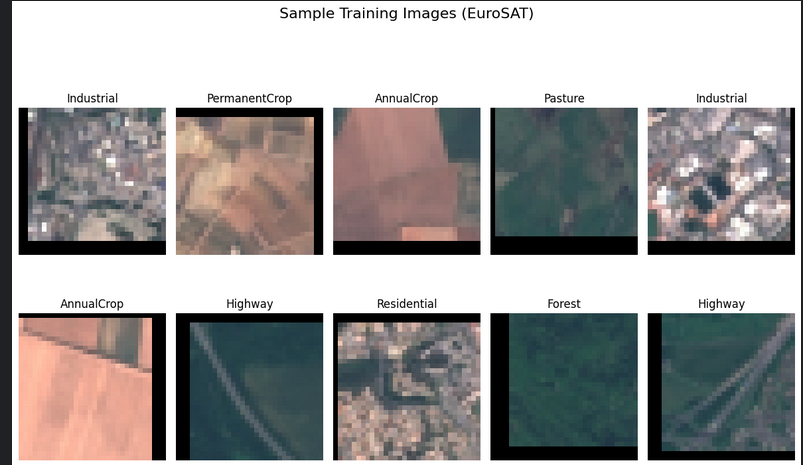
\includegraphics[width=0.95\textwidth]{sample_training_images.png}
    \caption{Sample images from the EuroSAT training dataset after initial preprocessing, displayed with their corresponding class labels. Images are denormalized for visualization.}
    \label{fig:eurosat_samples}
\end{figure}

\subsection{Model Architecture: ResNet-32}
The model implemented in this project is a ResNet-32 architecture, specifically adapted for $32 \times 32$ input images, drawing from the design principles outlined by He et al. for CIFAR-10 \cite{he2015deepresiduallearningimage}.

\subsubsection{Building Block: BasicBlock}
The network is constructed using the "BasicBlock" variant of residual blocks. Each BasicBlock consists of:
\begin{itemize}[itemsep=0.3em]
    \item Two sequential $3 \times 3$ convolutional layers.
    \item Batch Normalization (BN) applied after each convolutional layer.
    \item A ReLU activation function following the first BN layer.
    \item A shortcut connection that adds the input of the block ($x$) to the output of the second BN layer.
    \item A final ReLU activation applied after this addition.
\end{itemize}
The `expansion` factor for a BasicBlock is 1, meaning the number of output channels from the block is the same as the number of `planes` (filters) in its convolutional layers.

\subsubsection{Shortcut Connections}
\begin{itemize}[itemsep=0.3em]
    \item \textbf{Identity Shortcut:} If the input dimensions (spatial size and number of channels) to a BasicBlock match the output dimensions, the shortcut connection is a direct identity mapping.
    \item \textbf{Projection Shortcut:} If dimensions change (due to a strided convolution for downsampling, or an increase in the number of filters between stages), the shortcut connection employs a $1 \times 1$ convolution (with appropriate stride and output channels) followed by BN to match the output dimensions of the main path before the element-wise addition.
\end{itemize}

\subsubsection{Overall ResNet-32 Structure}
The ResNet-32 is composed as follows:
\begin{enumerate}[label=\arabic*), itemsep=0.5em]
    \item \textbf{Initial Convolution (conv1):} A $3 \times 3$ convolutional layer with 16 filters, stride 1, and padding 1. This is followed by Batch Normalization and a ReLU activation. The input image size is $3 \times 32 \times 32$. Output feature map: $16 \times 32 \times 32$.
    \item \textbf{Layer 1 (Stage 1):} A stack of 5 BasicBlocks. Each block uses 16 filters. The input to this stage is $16 \times 32 \times 32$. All blocks in this stage use stride 1. Output feature map: $16 \times 32 \times 32$.
    \item \textbf{Layer 2 (Stage 2):} A stack of 5 BasicBlocks. Each block uses 32 filters. The first BasicBlock in this stage uses a stride of 2 in its first convolutional layer (and its projection shortcut, if needed) for downsampling. Subsequent blocks in this stage use stride 1. Input feature map: $16 \times 32 \times 32$. Output feature map: $32 \times 16 \times 16$.
    \item \textbf{Layer 3 (Stage 3):} A stack of 5 BasicBlocks. Each block uses 64 filters. Similar to Layer 2, the first BasicBlock here uses a stride of 2 for downsampling. Input feature map: $32 \times 16 \times 16$. Output feature map: $64 \times 8 \times 8$.
    \item \textbf{Global Average Pooling:} An `nn.AdaptiveAvgPool2d((1, 1))` layer is applied to the output of Layer 3. This reduces each $64 \times 8 \times 8$ feature map to $64 \times 1 \times 1$.
    \item \textbf{Dropout:} A dropout layer with a rate of 0.25 is applied after pooling to provide regularization.
    \item \textbf{Classification Layer (Linear):} A fully connected linear layer maps the 64 features (from the 64x1x1 pooled output) to 10 output units, corresponding to the `NUM_CLASSES` in EuroSAT.
\end{enumerate}
The name "ResNet-32" comes from the count of weighted layers: 1 (initial conv1) + (5 blocks/stage $\times$ 2 convs/block $\times$ 3 stages) + 1 (linear layer) = $1 + 30 + 1 = 32$ layers.

\subsection{Training Procedure}
The ResNet-32 model was trained using the following configuration:
\begin{itemize}[itemsep=0.5em]
    \item \textbf{Loss Function:} `nn.CrossEntropyLoss`, suitable for multi-class classification.
    \item \textbf{Optimizer:} Stochastic Gradient Descent (SGD) with a momentum of 0.9 and L2 weight decay of $5 \times 10^{-4}$.
    \item \textbf{Learning Rate (LR) Strategy:}
        \begin{itemize}[itemsep=0.3em]
            \item \textit{Warmup:} A linear LR warmup was applied for the first `WARMUP_EPOCHS = 3` epochs. The LR started at `WARMUP_START_LR = 1 \times 10^{-5}` and linearly increased to `TARGET_INITIAL_LR = 0.01`.
            \item \textit{Scheduling:} After warmup, a `ReduceLROnPlateau` scheduler monitored the validation loss. If the validation loss did not improve for `PATIENCE_LR_SCHEDULER = 5` epochs, the LR was reduced by a factor of `FACTOR_LR_SCHEDULER = 0.2`. The minimum LR was $1 \times 10^{-6}$.
        \end{itemize}
    \item \textbf{Batch Size:} 128 images.
    \item \textbf{Epochs:} Maximum of `MAX_EPOCHS = 35`.
    \item \textbf{Early Stopping:} Training terminated if validation loss did not improve for `PATIENCE_EARLY_STOPPING = 10` epochs.
    \item \textbf{Best Model Saving:} The model state achieving the lowest validation loss was saved.
    \item \textbf{Device:} Training utilized a CUDA-enabled GPU.
\end{itemize}

\clearpage % Start new page for Section 4
\section{Results and Analysis}
The performance of the ResNet-32 model was tracked throughout the training process and subsequently evaluated on the held-out test set.

\subsection{Training Dynamics}
The training progress, including loss and accuracy metrics for both training and validation sets, along with the learning rate evolution, is illustrated in Figure \ref{fig:training_plots}.

\begin{figure}[H]
    \centering
    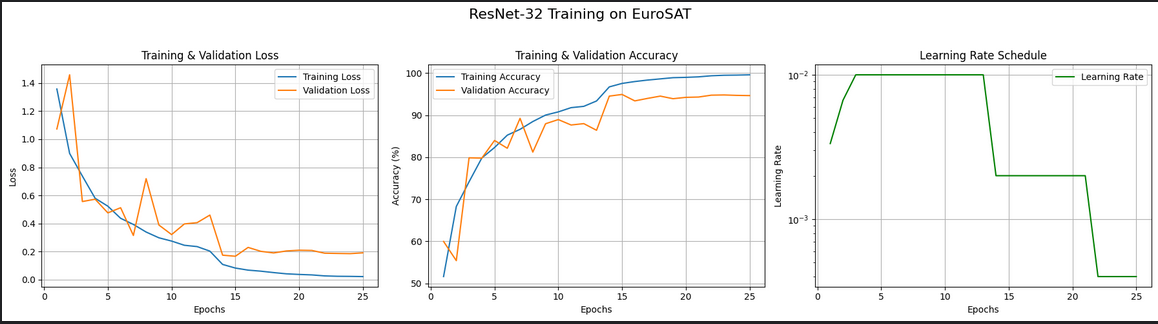
\includegraphics[width=\textwidth]{resnet32_eurosat_training_summary.png}
    \caption{ResNet-32 Training on EuroSAT: (Left) Training and Validation Loss over epochs. (Middle) Training and Validation Accuracy over epochs. (Right) Learning Rate schedule during training.}
    \label{fig:training_plots}
\end{figure}

\textbf{Observations from Training Curves:}
\begin{itemize}[itemsep=0.5em]
    \item \textbf{Initial Phase \& Warmup (Epochs 1-3):} The learning rate warmup successfully stabilized the initial training phase.
    \item \textbf{Mid-Training (Epochs 4-~14):} The model learned effectively at the target initial LR of 0.01.
    \item \textbf{First LR Reduction (Around Epoch 14):} The scheduler reduced LR (0.01 to 0.002), significantly improving validation accuracy (above 90\%) and lowering validation loss.
    \item \textbf{Second LR Reduction (Around Epoch 22):} LR dropped again (0.002 to 0.0004), leading to further fine-tuning. Training accuracy neared 100\%.
    \item \textbf{Convergence and Early Stopping:} Validation loss plateaued. Training halted at epoch 25 due to early stopping.
\end{itemize}

\textbf{Key Performance Metrics from Training Output (based on your PDF):}
\begin{itemize}[itemsep=0.3em]
    \item Total training time: 3.61 minutes (216.55 seconds).
    \item Best validation loss achieved during training: 0.1661.
    \item Best validation accuracy achieved during training: 94.91\% at epoch 15.
    \item Early stopping triggered after 25 epochs.
\end{itemize}

\subsection{Test Set Performance}
The model weights corresponding to the best validation loss (0.1661, from epoch 15) were loaded for evaluation on the unseen EuroSAT test set.
\begin{itemize}[itemsep=0.3em]
    \item \textbf{Final Test Loss:} 0.2027
    \item \textbf{Final Test Accuracy:} 93.93\%
\end{itemize}
The test accuracy is commendably high and close to the best validation accuracy, indicating good model generalization.

\subsection{Sample Predictions}
To qualitatively assess performance, predictions were made on test set images. Figure \ref{fig:sample_predictions} displays these.

\begin{figure}[H]
    \centering
    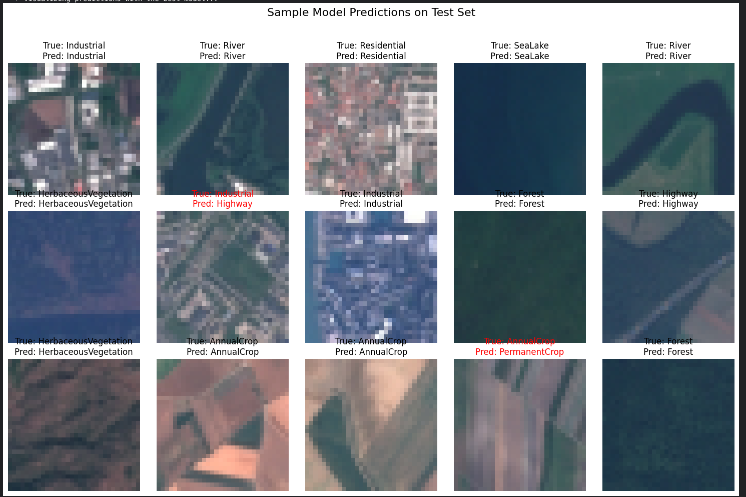
\includegraphics[width=0.95\textwidth]{sample_model_predictions.png}
    \caption{Sample model predictions on the EuroSAT test set. Each image shows "True: [True Label]" and "Pred: [Predicted Label]". Incorrect predictions are indicated by red text for the predicted label.}
    \label{fig:sample_predictions}
\end{figure}
The model correctly classifies many diverse images. Misclassifications (e.g., "River" as "Highway") often occur between visually similar classes, potentially exacerbated by the $32 \times 32$ resolution.

\clearpage % Start new page for Section 5
\section{Discussion}
The ResNet-32 model achieved a strong test accuracy of 93.93\% on EuroSAT, demonstrating residual learning's effectiveness.

\textbf{Impact of Architecture and Training Strategies:}
\begin{itemize}[itemsep=0.5em]
    \item Residual connections were vital for stable training of this 32-layer network.
    \item Learning rate warmup was crucial for stabilizing initial epochs.
    \item `ReduceLROnPlateau` effectively fine-tuned learning by adapting the LR.
    \item Early stopping based on validation loss selected a well-generalizing model, preventing overfitting despite training accuracy reaching near 100\%. The small gap between best validation (94.91\%) and final test accuracy (93.93\%) confirms this.
\end{itemize}

\textbf{Overfitting and Generalization:}
The typical gap between high training accuracy and slightly lower validation/test accuracy was observed. However, validation loss did not degrade after reaching its minimum, indicating that regularization (weight decay, dropout) and early stopping effectively controlled detrimental overfitting.

\textbf{Potential Further Improvements:}
\begin{enumerate}[itemsep=0.3em]
    \item \textbf{Dataset-specific Normalization:} Could offer minor gains.
    \item \textbf{Advanced Data Augmentation:} E.g., color jitter, rotations, MixUp \cite{Zhang2018Mixup}, CutMix \cite{Yun2019CutMix}.
    \item \textbf{Hyperparameter Optimization:} E.g., AdamW optimizer \cite{Loshchilov2019AdamW}.
    \item \textbf{Input Resolution/Model Scaling:} Using $64 \times 64$ inputs with an adapted ResNet.
    \item \textbf{Transfer Learning:} Fine-tuning an ImageNet pre-trained ResNet.
\end{enumerate}

\clearpage % Start new page for Section 6
\section{Conclusion}
This project successfully implemented a ResNet-32 architecture for EuroSAT image classification, achieving a test accuracy of 93.93\%. This result was facilitated by the core principles of deep residual learning and effective training strategies, including learning rate warmup, adaptive LR scheduling, and early stopping. The model demonstrated robust performance and good generalization. The detailed analysis of training dynamics provides a solid foundation and suggests avenues for further research in satellite image classification using residual networks.

\clearpage % Start new page for References
\printbibliography

\end{document}
